\documentclass[dvipsnames,border=3pt]{standalone}
\usepackage{tikz}
\usetikzlibrary{arrows}
\usetikzlibrary{shapes}
\usepackage{enumitem}
\usepackage{bm}
\usepackage{mathdots}
\usepackage{amsmath}
\usetikzlibrary{shadings}
\usetikzlibrary{decorations.pathreplacing}
\usepackage{helvet}
\usetikzlibrary{arrows.meta}
\usepackage{graphicx}
\usepackage{pgfplots}
\usepackage{pgfplotstable}
\usepackage{filecontents}
\usetikzlibrary{plotmarks}
\pgfplotsset{compat=newest}

\renewcommand{\familydefault}{\sfdefault}

\definecolor{mylightgray}{cmyk}{0,0,0,0.1}
\usetikzlibrary{arrows,decorations.pathmorphing,backgrounds,fit,positioning,shapes.symbols,chains}

\begin{document}

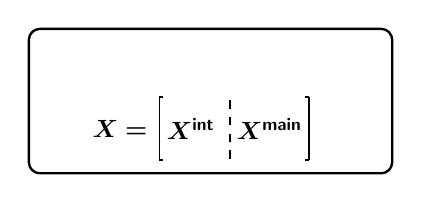
\begin{tikzpicture}
    % trim=left botm right top
    
    %%%%%%%%%%%%%%%%%%%%%%%%%%%%%%%%%%%%%%%%%%%%%%%%%%%%%%%%%%%%%%%%%%%%%%%%%%%%%%%%%%%%%%%%%%%%%%%%%%
    %%%%%%%%%%%%%%%%%%%%%%%%%%%%%%%%%%%%%%%%%%% box 7 %%%%%%%%%%%%%%%%%%%%%%%%%%%%%%%%%%%%%%%%%%%%%%%%
    %%%%%%%%%%%%%%%%%%%%%%%%%%%%%%%%%%%%%%%%%%%%%%%%%%%%%%%%%%%%%%%%%%%%%%%%%%%%%%%%%%%%%%%%%%%%%%%%%%
    
    \node[draw, rounded corners=4, line width=0.3mm, text width=4.38cm, text height=1.6cm] at (9.2,-9.75) {};
    %\node[circle,draw,line width=0.2mm,xscale=1.2,yscale=1.2,fill=GreenYellow] at (7,-7.6) {};
    %\node at (7,-7.6) {\textbf{5}};
    
    %%%%%%%%%%%%%%%%%%%%%%%%%%%%%%%%%%%%%%%%%%%%%%%%%%%%%%%%%%%%%%%%%%%%%%%%%%%%%%%%%%%%%%%%%%%%%%%%%%
    %%%%%%%%%%%%%%%%%%%%%%%%%%%%%%%%%%%%%%%%%%% box 7 %%%%%%%%%%%%%%%%%%%%%%%%%%%%%%%%%%%%%%%%%%%%%%%%
    %%%%%%%%%%%%%%%%%%%%%%%%%%%%%%%%%%%%%%%%%%%%%%%%%%%%%%%%%%%%%%%%%%%%%%%%%%%%%%%%%%%%%%%%%%%%%%%%%%
    
    %%%%%%%%%%%%%%%%%%%%%%%%%%%%%%%%%%%%%%%%%%%%%%%%%%%%%%%%%%%%%%%%%%%%%%%%%%%%%%%%%%%%%%%%%%%%%%%%%%
    %%%%%%%%%%%%%%%%%%%%%%%%%%%%%%%%%%%%%%% correlated data %%%%%%%%%%%%%%%%%%%%%%%%%%%%%%%%%%%%%%%%%%
    %%%%%%%%%%%%%%%%%%%%%%%%%%%%%%%%%%%%%%%%%%%%%%%%%%%%%%%%%%%%%%%%%%%%%%%%%%%%%%%%%%%%%%%%%%%%%%%%%%
    %\node[draw,rounded corners=2,line width=0.2mm,fill=gray!50,text height=0.3cm, text width=2.57cm,shading angle=45] at (9.5,-7.65) {}; % random graph
    %\node at (9.5,-7.65) {\textbf{Correlated Data}};
    
    
    \node[xscale=0.9,yscale=0.9] at (8.05,-10.1) {\bm{$X =$}};
    \draw[line width=0.2mm] (8.55,-10.5) -- (8.55,-9.7);
    \draw[line width=0.2mm] (10.45,-10.5) -- (10.45,-9.7);
    
    \draw[line width=0.2mm] (8.55,-10.5) -- (8.6,-10.5);
    \draw[line width=0.2mm] (8.55,-9.7) -- (8.6,-9.7);
    
    \draw[line width=0.2mm] (10.45,-10.5) -- (10.4,-10.5);
    \draw[line width=0.2mm] (10.45,-9.7) -- (10.4,-9.7);
    
    \draw[line width=0.2mm,dashed] (9.45,-10.48) -- (9.45,-9.7);
    
    \node[xscale=0.9,yscale=0.9] at (8.95,-10.1) {\bm{$X^\textbf{int}$}};
    \node[xscale=0.9,yscale=0.9] at (9.95,-10.1) {\bm{$X^\textbf{main}$}};
    %%%%%%%%%%%%%%%%%%%%%%%%%%%%%%%%%%%%%%%%%%%%%%%%%%%%%%%%%%%%%%%%%%%%%%%%%%%%%%%%%%%%%%%%%%%%%%%%%%
    %%%%%%%%%%%%%%%%%%%%%%%%%%%%%%%%%%%%%%% correlated data %%%%%%%%%%%%%%%%%%%%%%%%%%%%%%%%%%%%%%%%%%
    %%%%%%%%%%%%%%%%%%%%%%%%%%%%%%%%%%%%%%%%%%%%%%%%%%%%%%%%%%%%%%%%%%%%%%%%%%%%%%%%%%%%%%%%%%%%%%%%%%
    
    \end{tikzpicture}
    
\end{document}